\graphicspath{{./figures}}

\section{Full System}

The South African Weather Service kindly granted permission to track their weather balloons, which contain Radiosondes. This allowed for a tracking system test to be conducted, with focus on closed-loop tracking. The system computer unfortunately lost power near the 25 km mark, and a second test could not be conducted due to time constraints. However, it was observed that the mount correctly steered the antenna based on the received GPS data. The results of both the predicted path and the actual path for the weather balloon, as well as the recorded SNR as a function of distance, are shown in Figures \ref{fig:radiosondePredictedVsActual} and \ref{fig:radiosondeSnr}.

\begin{figure}[!htb]
  \begin{minipage}{.4\textwidth}
    \centering
    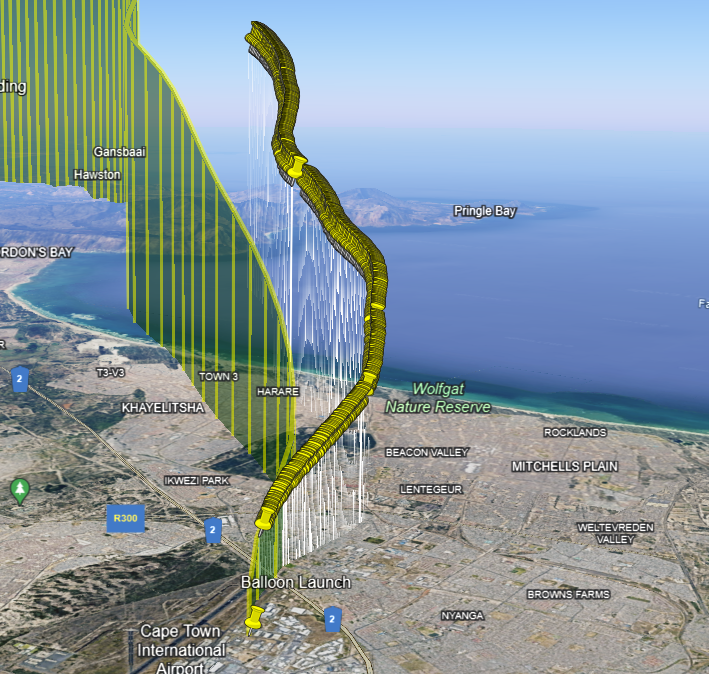
\includegraphics[width=0.85\linewidth]{radiosondePredictedVsActual}
    \caption{Radiosonde Closed-Loop Tracking Predicted Path (left) vs Actual (right)}
    \label{fig:radiosondePredictedVsActual}
  \end{minipage}
  \begin{minipage}{.6\textwidth}
    \centering
    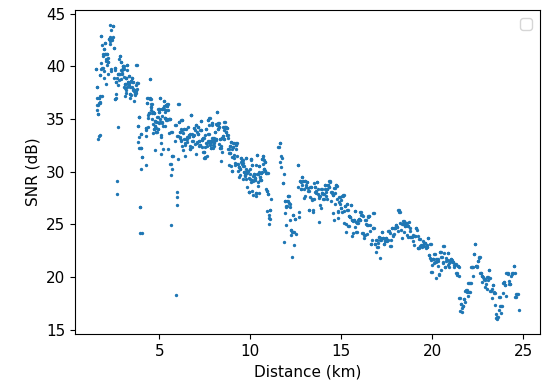
\includegraphics[width=0.95\linewidth]{radiosondeSnr}
    \caption{Radiosonde Closed-Loop Tracking SNR vs Distance}
    \label{fig:radiosondeSnr}
  \end{minipage}
\end{figure}